\chapter{Einführung}

\section{Motivation}

Die Entwicklung und Verbesserung von Frameworks zur Verarbeitung großer Datenmengen ist zur Zeit hochaktuell und im Fokus von Medien und Unternehmen angekommen \cite{Bit14}. Verschiedene Programme und Paradigmen konkurrieren um die schnellste, bequemste und stabilste Art großen Datenmengen einen geschäftsfördernden Nutzen abzuringen \cite{Sin14}.\\

Mit dem Begriff "`große Datenmengen"' oder "`Big Data"' werden in dieser Arbeit solche Datenmengen zusammengefasst, die die Kriterien Volume, Velocity, Variety \cite{Lan01} erfüllen oder "`Datenmengen, die nicht mehr unter Auflage bestimmter \gls{sla}s auf einzelnen Maschinen verarbeitet werden können"' (Vgl. \cite{Sam14}).\\

Als Unternehmen, das früh mit zeitkritischen Aufgaben (u.a.  Indizierung von Webseiten und PageRank \cite{page2001method}) auf solchen Datenmengen konfrontiert war implementierte Google das Map-Reduce Paradigma \cite{Dean04} als Framework zur Ausnutzung vieler kostengünstiger Rechner für verschiedene Aufgaben. \\

In Folge der Veröffentlichung dieser Idee im Jahr 2004 wurde Map-Reduce in Form der OpenSource Implementation Hadoop (gemeinsam mit einer Implementation des Google File Systems GFS, u.a.) \cite{Ghema03} zum de-facto Standard für Big-Data-Analyseaufgaben.\\

Reines Map-Reduce (in der ursprünglichen Implemenation von Hadoop) als Berechnungsparadigma zur Verarbeitung großer Datenmengen zeigt jedoch in vielen Anwendungsfällen Schwächen:
\begin{itemize}
	\item Daten, die in hoher Frequenz entstehen und schnell verarbeitet werden sollen erfordern häufiges Neustarten von Map-Reduce-Jobs. Die Folge ist kostspieliger Overhead durch Verwaltung/Scheduling der Jobs und gegebenenfalls wiederholtem Einlesen von Daten.
	\item Algorithmen die während ihrer Ausführung iterativ Zwischenergebnisse erzeugen und auf vorherige angewiesen sind (häufig bei Maschinenlernalgorithmen) können nur durch persistentes Speichern der Daten und wiederholtes Einlesen zwischen allen Iterationsschritten implementiert werden.
	\item Anfragen an ein solches Map-Reduce-System erfolgen imperativ in Form von kleinen Programmen. Dieses Verfahren ist offensichtlich nicht so intuitiv und leicht erlernbar wie deklarative Abfragesprachen klassischer Datenbanken (z.B. SQL).
\end{itemize}

In der Folge dieser Probleme entstanden viele Ansätze dieses Paradigma zu ersetzen, zu ergänzen oder durch übergeordnete Ebenen und High-Level-APIs zu vereinfachen \cite{Sin14}.\\

Eine der Alternativen zu der klassischen Map-Reduce-Komponente in Hadoop ist die "`general engine for large-scale data processing"' Apache Spark.\\

Ein Indiz für das steigende Interesse an diesem Produkt liefert unter anderem ein Vergleich des Interesses an Hadoop und Spark auf Google:\\

\begin{figure}[h]
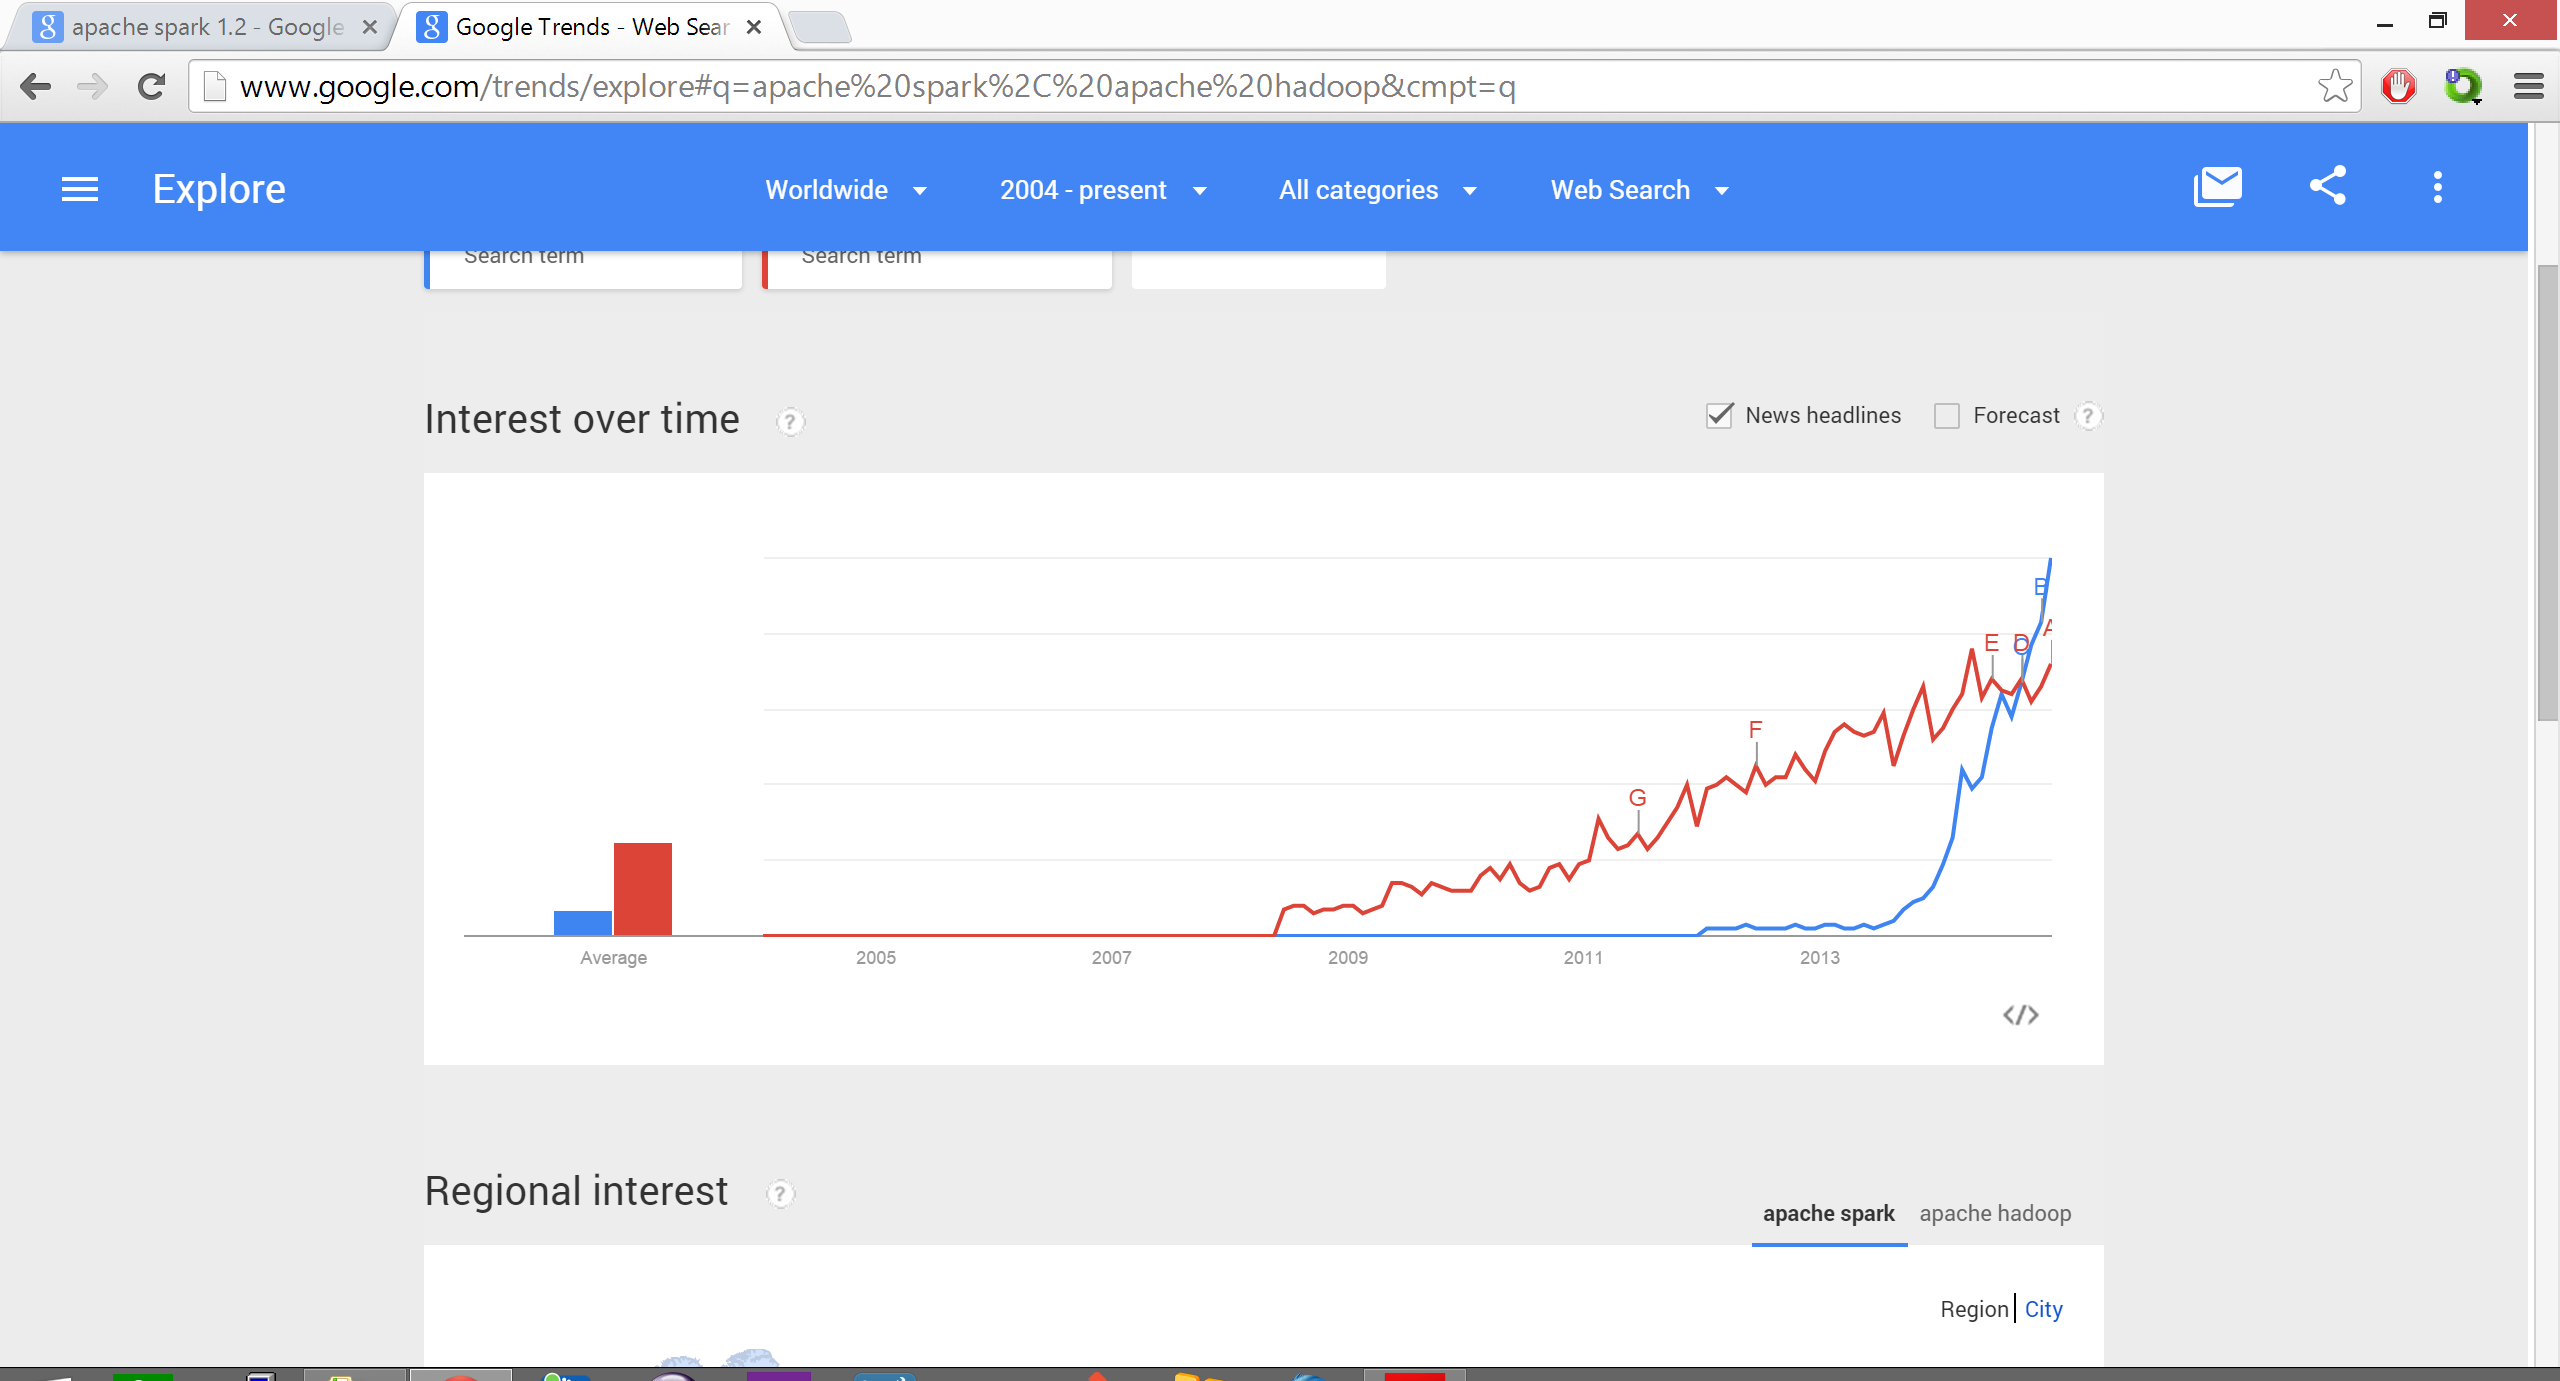
\includegraphics[width=0.9\textwidth]{bilder/trends_spark_vs_hadoop.PNG}
\caption[Google Trends]{Suchanfragen zu "`Apache Spark"' (\textit{blau}) und "`Apache Hadoop"' (\textit{rot}), Stand 24.03.2015 \cite{googletrends}}
\end{figure}

\section{Ziel dieser Arbeit}
Das Ziel dieser Arbeit ist es den Betrieb einer realitätsnahen Spark-Anwendung auf einem Cluster mit Hardware am unteren Ende des Leistungsspektrums zu begutachten.\\
Dabei wird zunächst ein umfassender Überblick der grundlegenden Konzepte von Spark gegeben. Anschließend wird ein Anwendungsfall aus dem Bereich des Text-Mining vorgestellt und dessen Realisierung vom Entwurf bis zum Betrieb erläutert.\\

Der theoretische Teil dieser Arbeit umfasst
\begin{itemize}
  \item eine Einführung in die grundlegenden Konzepte von Apache Spark 
	\item eine kurze Einordnung von Spark durch den Vergleich mit ähnlichen Anwendungen
\end{itemize}

Der praktische Teil dieser Arbeit umfasst
\begin{itemize}
\item die Implementation einer hybriden Anwendung mit einer Echtzeitkomponente (Spark Streaming Library) und einer Batch-Komponente (Spark Machine Learning Library).
\item den Betrieb dieser Anwendung auf einem Cluster mit Hardware am unteren Ende des Leistungsspektrums.
\end{itemize}

Apache Spark ist überwiegend in der Programmiersprache Scala\footnote{http://www.scala-lang.org/, abgerufen am 03.03.2015} geschrieben. Die Beispiele in dieser Arbeit werden ebenfalls in Scala verfasst um
\begin{enumerate}
	\item einen einheitlichen Stil und Vergleichbarkeit zwischen Quellcode-Auszügen und eigenen Beispielen zu gewährleisten.
	\item Ausdrücke in kurzer, prägnanter Form darzustellen.
\end{enumerate}
